\documentclass[aspectratio=169]{beamer}
\usetheme{Madrid}
\usecolortheme{default}
\usefonttheme{professionalfonts}

\usepackage[utf8]{inputenc}
\usepackage[T1]{fontenc}
\usepackage[spanish,es-nodecimaldot]{babel}
\usepackage{lmodern}
\usepackage{ragged2e}
\usepackage{booktabs}
\usepackage{enumitem}
\usepackage{hyperref}
\usepackage{tikz}
\usetikzlibrary{shapes.geometric, arrows.meta, positioning, backgrounds, fit}
\graphicspath{{graficos_ppt/}}

\setbeamertemplate{navigation symbols}{}
\setbeamertemplate{footline}[frame number]
\setbeamertemplate{bibliography item}[text]

\newcommand{\smallrefs}[1]{{\tiny\color{gray} #1}}
\newcommand{\refcite}[1]{{\footnotesize\color{gray!70!black} #1}}

% ---------------------------------------------------------------------------
% Portada
% ---------------------------------------------------------------------------
\title{Propuesta de Investigación}
\subtitle{Trabajo de Investigación I\\MIA 3er Ciclo A 2026-1 $\cdot$ Grupo 9B}
\author{Luis Koc \and \\ Herbert Meléndez}
\date{\today}

% Diapositivas separadoras de sección
\AtBeginSection[]{%
  \begin{frame}[plain, noframenumbering]
    \vfill
    \centering
    \begin{beamercolorbox}[sep=12pt,center,shadow=true,rounded=true]{title}
      \usebeamerfont{title}\insertsectionhead\par%
    \end{beamercolorbox}
    \vfill
  \end{frame}
}

\begin{document}

\begin{frame}
  \titlepage
\end{frame}

% ---------------------------------------------------------------------------
% ESTRUCTURA
% ---------------------------------------------------------------------------
\begin{frame}{Estructura de la presentación}
\tableofcontents[hideallsubsections]
\end{frame}

% ===========================================================================
\section{Título tentativo e idea central}
% ===========================================================================

\begin{frame}{Título tentativo}

\begin{block}{}
\centering\large
\textbf{Efecto de la heterogeneidad térmica del entorno sobre la temperatura
del conductor en cables subterráneos: modelado numérico 2D y análisis de la
brecha normativa}
\par\vspace{0.35em}

\end{block}

\vspace{0.8em}
\begin{columns}[T]
\column{0.45\textwidth}
\textbf{Campo disciplinario}
\begin{itemize}[leftmargin=*]\small
    \item Sistemas eléctricos de potencia
    \item Transferencia de calor computacional
    \item Modelado numérico e IA aplicada
\end{itemize}
\column{0.50\textwidth}
\textbf{Etapa del proceso investigativo}
\begin{itemize}[leftmargin=*]\small
    \item Comprensión y formulación del problema
    \item Identificación de la brecha
    \item Esbozo de posibles soluciones
\end{itemize}
\end{columns}
\end{frame}

% ---------------------------------------------------------------------------
\begin{frame}{Idea central}
\justifying

\begin{alertblock}{¿Qué duele? (el problema)}
Los cables subterráneos se diseñan y operan con métodos que asumen condiciones
térmicas uniformes y estacionarias. Cuando el entorno real es heterogéneo,
dinámico o complejo, esos métodos pueden sobrestimar o subestimar la
temperatura real del conductor, generando riesgo de falla o subutilización
de infraestructura crítica.
\end{alertblock}

\vspace{0.5em}
\begin{columns}[T]
\column{0.23\textwidth}
\begin{block}{\small¿Qué?}
\tiny Brecha entre modelos simplificados y la realidad térmica del cable
\end{block}
\column{0.23\textwidth}
\begin{block}{\small¿Dónde?}
\tiny Cables enterrados en ciudades, parques solares y eólicos
\end{block}
\column{0.23\textwidth}
\begin{block}{\small¿Por qué?}
\tiny El suelo, el relleno y la geometría son heterogéneos y variables
\end{block}
\column{0.23\textwidth}
\begin{block}{\small¿Para qué?}
\tiny Operar más seguro, evitar fallas y aprovechar mejor la capacidad
\end{block}
\end{columns}

\vspace{0.4em}
\refcite{Referencias base: (Neher y McGrath, 1957); (IEC 60287-1-1, 2023);
(Aras et al., 2005); (Kim et al., 2025)}
\end{frame}

% ===========================================================================
\section{El cable y su entorno de instalación}
% ===========================================================================

\begin{frame}{Cables subterráneos: infraestructura crítica sin margen de error}
\begin{columns}[T]
\column{0.52\textwidth}
\justifying\small
Los cables eléctricos subterráneos sostienen la transmisión y distribución en
zonas urbanas donde la red aérea es inviable. Además son la única vía de
evacuación de energía en parques solares y eólicos.

\vspace{0.5em}
\textbf{¿Qué ocurre cuando fallan?}
\begin{itemize}[leftmargin=*]\small
    \item Reparación: \textbf{semanas a meses} (excavación, empalmes, pruebas
          dieléctricas, normalización)
    \item En sistemas sin redundancia: corte total de suministro
    \item Impacto en hospitales, agua potable, plantas industriales
    \item Para renovables: toda la generación queda inactiva hasta la
          reparación
    \item Se convierte en \textbf{cuello de botella} para la transición
          energética
\end{itemize}

\vspace{0.4em}
\refcite{(Fariz et al., 2026, p.~1); (Möbius et al., 2025, p.~1);
(Enescu et al., 2021, p.~2)}

\column{0.44\textwidth}
\begin{tikzpicture}[>=Stealth,
  box/.style={draw, rounded corners, align=center, font=\tiny,
              minimum height=0.85cm, text width=2.4cm, inner sep=4pt}]

  % Fila 1: subestación
  \node[box, fill=yellow!30] (sub) at (0, 5.4) {Subestación\\de transmisión};

  % Fila 2: cable
  \node[box, fill=gray!25] (cable) at (0, 4.1)
        {Cable\\subterráneo\\(tramo único)};

  % Fila 3: consumidores (izq y der), bien separados
  \node[box, fill=blue!15]  (ciudad) at (-2.0, 2.5) {Red\\urbana};
  \node[box, fill=green!15] (solar)  at ( 2.0, 2.5) {Parque\\solar/eólico};

  % Fila 4: falla (debajo del cable, entre los anteriores)
  \node[box, fill=red!15, draw=red!70!black, dashed] (falla) at (0, 0.5)
        {\textbf{Falla}\\semanas\\sin servicio};

  % Flechas
  \draw[->, thick] (sub.south)       -- (cable.north);
  \draw[->, thick] (cable.south west) to[out=240,in=90] (ciudad.north);
  \draw[->, thick] (cable.south east) to[out=300,in=90] (solar.north);
  \draw[->, thick, red!70!black, dashed] (cable.south) -- (falla.north);

  % Nota
  \node[font=\tiny, gray] at (0,-0.35) {Sin redundancia = impacto total};
\end{tikzpicture}
\end{columns}
\end{frame}

% ---------------------------------------------------------------------------
\begin{frame}{Estructura interna de un cable subterráneo de potencia}
\begin{columns}[T]
\column{0.52\textwidth}
\justifying\small
Un cable de alta tensión está formado por capas concéntricas con
funciones eléctricas y térmicas bien definidas
\refcite{(Thue, 2012; IEC~60287-1-1, 2023)}:
\begin{itemize}[leftmargin=*]\scriptsize
    \item \textbf{Conductor} (Cu o Al, 95--1\,200~mm²): fuente primaria de
          calor por efecto Joule; $k_\text{Cu}\approx 385$~W/(m\,K).
    \item \textbf{Capas semiconductoras}: uniformizan el campo eléctrico;
          barrera térmica adicional, $k\approx 0{,}3$~W/(m\,K).
    \item \textbf{Aislamiento XLPE}: barrera térmica principal;
          $k\approx 0{,}286$~W/(m\,K); $T_{\max}=90$~\textdegree{}C en
          servicio continuo, 250~\textdegree{}C en cortocircuito.
    \item \textbf{Pantalla metálica} (cinta de Cu/Al): fuente secundaria
          de calor por corrientes de apantallamiento inducidas.
    \item \textbf{Cubierta exterior} (PE o PVC): protección mecánica y
          contra humedad; $k\approx 0{,}2$--$0{,}4$~W/(m\,K).
\end{itemize}

\column{0.44\textwidth}
\centering
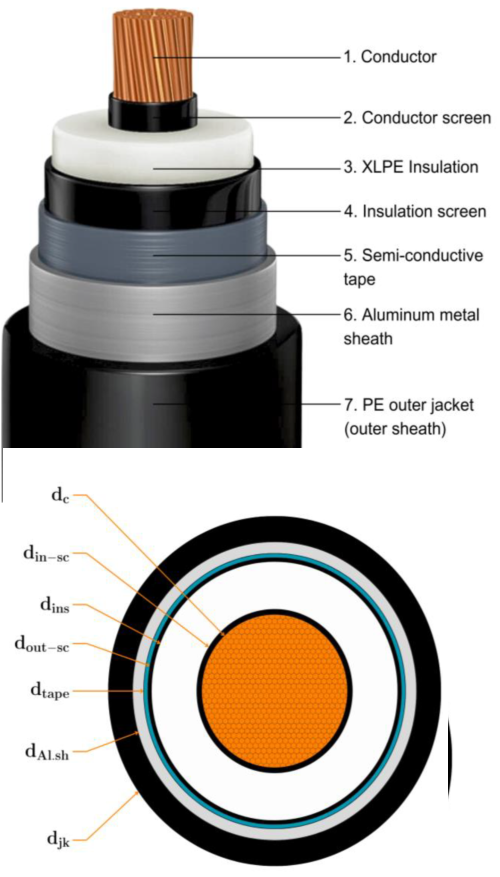
\includegraphics[width=0.94\linewidth]{kim2025_cable_xsection}\\
{\tiny\color{gray} Sección transversal cable XLPE 154~kV (7 capas concéntricas).\\
\refcite{Kim et al.\ (2025) [R5]}}
\vspace{0.2em}
\begin{alertblock}{}\scriptsize
La resistividad térmica del suelo ($\rho_T = 1/k$) es el parámetro de
mayor incertidumbre. Variaciones entre 0{,}5 y 2{,}5~K\,m/W pueden
modificar la ampacidad en más del 20\,\%.
\refcite{(Thue, 2012; Khumalo et al., 2025)}
\end{alertblock}
\end{columns}
\end{frame}

% ---------------------------------------------------------------------------
\begin{frame}{El entorno de instalación: zanja, bedding y backfill}
\begin{columns}[T]
\column{0.54\textwidth}
\justifying\small
El cable no opera solo: está integrado en un \textbf{sistema de instalación}
cuyo diseño determina cómo se disipa el calor
\refcite{(Ocłoń et al., 2015; Kim et al., 2025; Thue, 2012)}:
\begin{itemize}[leftmargin=*]\scriptsize
    \item \textbf{Profundidad de enterramiento} ($z$): típicamente 0{,}8--1{,}5~m.
          Mayor profundidad implica $T_\text{suelo}$ más estable pero trayecto de
          disipación más largo hacia la superficie.
    \item \textbf{Bedding (lecho)}: capa de arena fina ($\pm$15~cm) que rodea
          directamente al cable. Su $k$ es la \emph{primera resistencia térmica}
          entre cable y suelo: domina el gradiente $\Delta T$ en la zona próxima.
    \item \textbf{Backfill (relleno)}: material con el que se rellena la zanja
          sobre el bedding. Puede ser tierra excavada (variable, $k$ incierto)
          o material granular seleccionado.
    \item \textbf{Thermal backfill / FTB}: mezclas de arena, cemento y agua
          diseñadas para maximizar $k$ en la zona de influencia térmica del cable;
          reducen $T_\text{cond}$ y aumentan la ampacidad sin cambiar el cable.
\end{itemize}
\column{0.42\textwidth}
\centering
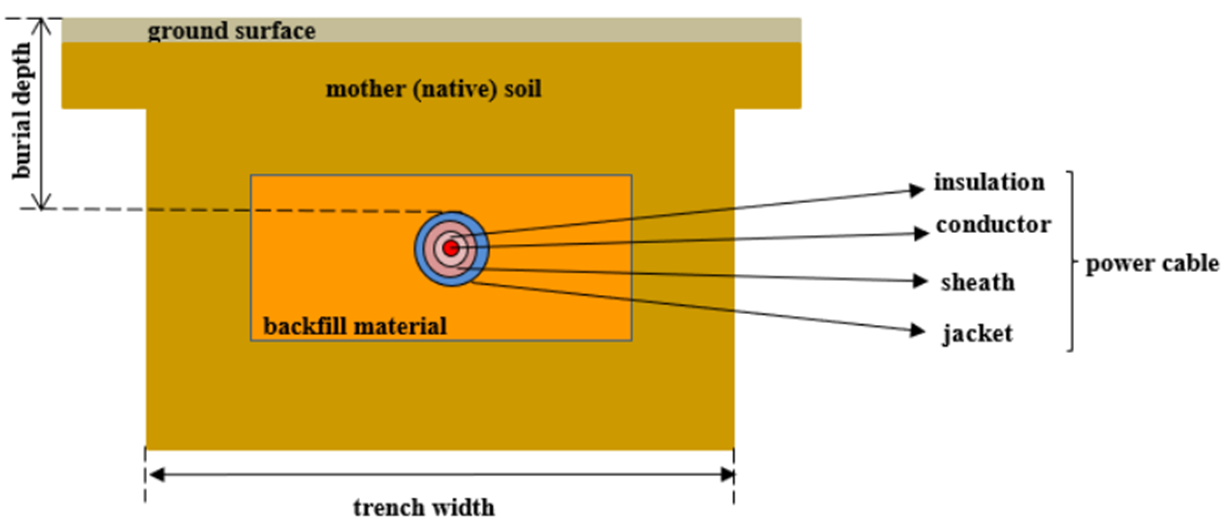
\includegraphics[width=\linewidth]{enescu_trench_xsection}\\
{\tiny\color{gray} Cable enterrado en backfill: sección transversal de zanja.\\
\refcite{Enescu et al.\ (2021) [R7]}}
\vspace{0.2em}
\begin{exampleblock}{}\scriptsize
Optimizar el bedding es una palanca directa de diseño para
aumentar la ampacidad. IEC~60287 asume un $k$ único del medio:
no distingue entre bedding y suelo nativo.
\refcite{(Atoccsa et al., 2024; Kim et al., 2025)}
\end{exampleblock}
\end{columns}
\end{frame}

% ---------------------------------------------------------------------------
\begin{frame}{El suelo como medio térmico: variabilidad y estratificación}
\begin{columns}[T]
\column{0.50\textwidth}
\justifying\small
El suelo \textbf{no es un material uniforme}. Su conductividad térmica $k$
varia con la composición mineral, el contenido de humedad, la compactación
y la temperatura \refcite{(Kolawole et al., 2024; Anders, 2005)}:
\begin{itemize}[leftmargin=*]\scriptsize
    \item \textbf{Composición mineral}: arena, arcilla, grava, roca; cada
          material tiene $k$ distinta (arena seca $\approx0{,}3$; roca
          calcárea $\approx2{,}5$~W/(m\,K)).
    \item \textbf{Humedad}: el agua intersticial incrementa fuertemente $k$.
          Un suelo saturado puede tener $k$ 4--6 veces mayor que el mismo
          suelo seco.
    \item \textbf{Compactación}: mayor densidad aparente $\to$ mayor contacto
          entre partículas $\to$ mayor $k$.
    \item \textbf{Estratificación real}: el suelo tiene capas de distinta
          composición a lo largo de la profundidad y de la ruta del cable.
          En entornos urbanos suele ser material de relleno heterogéneo
          (escombros, arenas, suelos intervenidos).
    \item \textbf{Consecuencia}: $k=k(x,y)$ es verdaderamente variable en
          el espacio; la hipótesis $k=\text{const}$ de IEC~60287 puede ser
          muy imprecisa.
\end{itemize}

\column{0.46\textwidth}
\small\textbf{Rangos típicos de $k$ del suelo}
\vspace{0.15em}
\begin{center}\scriptsize
\begin{tabular}{lc}
\toprule
\textbf{Tipo / condición}         & \textbf{$k$ (W/m\,K)} \\
\midrule
Arena seca                         & 0{,}25--0{,}35 \\
Arena húmeda                       & 1{,}0--2{,}0 \\
Arcilla seca                       & 0{,}4--0{,}5 \\
Arcilla saturada                   & 1{,}4--1{,}8 \\
Suelo urbano (relleno mixto)       & 0{,}5--1{,}5 \\
Roca calcárea                      & 2{,}0--3{,}0 \\
\bottomrule
\end{tabular}
\end{center}
\vspace{0.2em}
\begin{alertblock}{}\scriptsize
Variaciones de $k$ de hasta 5$\times$ pueden ocurrir a lo largo de
un mismo tramo de cable, generando cuellos de botella térmicos
localizados que los modelos uniformes no predicen.
\refcite{(Kolawole et al., 2024; Khumalo et al., 2025)}
\end{alertblock}
\end{columns}
\end{frame}

% ---------------------------------------------------------------------------
\begin{frame}{Factores dinámicos: ciclos de carga y secado térmico}
\begin{columns}[T]
\column{0.50\textwidth}
\textbf{\small Ciclos de carga $I(t)$ y temperatura del suelo}
\begin{itemize}[leftmargin=*]\scriptsize
    \item \textbf{Ciclo diario}: pico en horas punta; reducción nocturna.
          El cable sube y baja cíclicamente de temperatura.
    \item \textbf{Estacional}: mayor demanda en verano coincide con mayor
          $T_\text{amb}$ --- peor caso térmico combinado.
    \item \textbf{Solar}: carga nula de noche, pico al mediodía; ciclos
          marcados y predecibles.
    \item \textbf{Eólica}: carga estocástica y variable; el cable no
          alcanza equilibrio estacionario.
    \item \textbf{Sobrecargas}: corrientes sobre el nominal por períodos
          cortos, críticas para el aislamiento XLPE.
\end{itemize}
\vspace{0.2em}
\begin{itemize}[leftmargin=*]\scriptsize
    \item Superficie del suelo: 5--35~\textdegree{}C (zona templada).
    \item A 0{,}8~m: amplitud estacional atenuada $\approx$50\,\%,
          desfase 4--6 semanas.
    \item A $>$2~m: prácticamente constante en la media anual del sitio.
    \refcite{(Möbius et al., 2025; Kim et al., 2025)}
\end{itemize}
\column{0.46\textwidth}
\begin{alertblock}{\small Secado térmico: el riesgo oculto}
\scriptsize
Bajo carga sostenida elevada:
\begin{enumerate}[leftmargin=*,itemsep=0pt]
    \item $T_\text{suelo}>50$~\textdegree{}C cerca del cable.
    \item La humedad migra hacia zonas más frías.
    \item $k$ cae de $\approx$1{,}5 a $<$0{,}5~W/(m\,K).
    \item Resistencia térmica se triplica.
    \item $T_\text{cond}$ sube más $\to$ ciclo de retroalimentación.
    \item Ampacidad efectiva se reduce 20--30\,\%.
    \item El suelo seco \textbf{no se rehúmeda espontáneamente}.
\end{enumerate}
\refcite{(Khumalo et al., 2025, pp.~6--10; Anders, 2005)}
\end{alertblock}
\vspace{0.15em}
\begin{exampleblock}{}\scriptsize
IEC~60287 asume $T_\text{suelo}$ fija y carga al 100\,\%.
IEC~60853 corrige la carga cíclica pero no capta la variabilidad
espacial del entorno ni el secado en condiciones reales.
\refcite{(Enescu et al., 2021; Khumalo et al., 2025)}
\end{exampleblock}
\end{columns}
\end{frame}

% ---------------------------------------------------------------------------
\begin{frame}{Sensores y medios de recolección de datos térmicos}
\begin{columns}[T]
\column{0.48\textwidth}
\begin{block}{Sensores distribuidos de temperatura (DTS)}
\scriptsize\justifying
Tecnología de referencia para monitoreo continuo en cables de alta
tensión \refcite{(Li et al., 2006; Enescu et al., 2021)}:
\begin{itemize}[leftmargin=*,itemsep=1pt]
    \item Principio: dispersión Raman en fibra óptica embebida o
          co-instalada junto al cable.
    \item Resolución espacial: 0{,}5--2~m; alcance: hasta 30--50~km.
    \item Precisión: $\pm$0{,}1--0{,}5~\textdegree{}C; adquisición cada
          1--5~min.
    \item Localiza puntos calientes y cuellos de botella térmicos
          invisibles para sensores discretos.
\end{itemize}
\end{block}
\vspace{0.2em}
\begin{block}{Sensores puntuales}
\scriptsize
PT100/PT1000 o termopares en empalmes, subestaciones y cámaras.
Alta precisión ($\pm$0{,}1~\textdegree{}C) pero cobertura espacial
discreta; no revelan la distribución a lo largo del tendido.
\end{block}

\column{0.48\textwidth}
\centering

\vspace{0.2em}
\begin{block}{SCADA / plataformas DTR}
\scriptsize
Integran corriente, tensión, temperatura y datos ambientales para
calcular la ampacidad disponible en tiempo real
(\textit{Dynamic Thermal Rating}).
\refcite{(Fariz et al., 2026; Enescu et al., 2021)}
\end{block}
\vspace{1.5em}
\begin{alertblock}{Brecha de monitoreo}
\scriptsize
La mayoría de instalaciones no cuenta con DTS ni sensores de suelo.
El operador desconoce $T_\text{cond}$ y la distribución real de
$k(x,y)$ a lo largo del tendido.
\refcite{(Enescu et al., 2021, p.~14)}
\end{alertblock}
\end{columns}
\end{frame}

% ---------------------------------------------------------------------------
\begin{frame}{¿Qué determina la temperatura del conductor?}
\justifying\small
La temperatura en el conductor depende de la \textbf{disipación de calor hacia
el entorno}. Ese entorno \emph{no} es uniforme ni estático:

\vspace{0.2em}
\begin{columns}[T]
\column{0.48\textwidth}
\textbf{\small Variables del suelo y del medio}
\begin{itemize}[leftmargin=*]\scriptsize
    \item Conductividad térmica $k(x,y)$: varía con humedad,
          compactación y temperatura \refcite{(Kolawole et al., 2024)}
    \item Temperatura del suelo $T_s$ y del aire $T_\text{amb}$:
          estacional, profundidad \refcite{(Kim et al., 2025, pp.~3--5)}
    \item Secado térmico: la carga sostenida reduce la humedad local y
          eleva la resistividad
          \refcite{(Khumalo et al., 2025, pp.~4--6)}
\end{itemize}
\column{0.48\textwidth}
\textbf{\small Variables de instalación y operación}
\begin{itemize}[leftmargin=*]\scriptsize
    \item Material de relleno/bedding: $k$ entre 0.5 y 3.0 K·m/W
          \refcite{(Ocłoń et al., 2015)}
    \item Separación entre cables y agrupamientos
          \refcite{(Aras et al., 2005)}
    \item Profundidad de enterramiento $z$
    \item Perfil de carga $I(t)$: cíclico, variaciones rápidas, emergencias
          \refcite{(Enescu et al., 2021)}
    \item Cruces con tuberías u otras fuentes de calor
\end{itemize}
\end{columns}

\vspace{0.2em}
\begin{exampleblock}{}
\centering\small
Cuando estas variables se alejan de los supuestos normativos,
el modelo simplificado ya no predice bien la temperatura real del conductor.
\end{exampleblock}
\end{frame}

% ===========================================================================
\section{El problema físico}
% ===========================================================================

% ---------------------------------------------------------------------------
\begin{frame}{Física del problema: ecuación de conducción de calor}
\begin{columns}[T]
\column{0.8\textwidth}
\justifying\small
La temperatura está gobernada por la
\textbf{ecuación de conducción de calor 2D con coeficientes variables}
\refcite{(Carslaw \& Jaeger, 1959; Aras et al., 2005)}:
\begin{equation*}
\frac{\partial}{\partial x}\!\left(k\,\frac{\partial T}{\partial x}\right)+
\frac{\partial}{\partial y}\!\left(k\,\frac{\partial T}{\partial y}\right)
+Q = \rho c_p\,\frac{\partial T}{\partial t}
\end{equation*}
\begin{block}{Variables clave}
\scriptsize
\begin{itemize}[leftmargin=*,itemsep=1pt]
    \item $k(x,y)$: conductividad térmica variable en conductor, XLPE,
          relleno y suelo.
    \item $Q(x,y)$: fuente de calor (W/m\textsuperscript{3});
          activa en conductor ($I^2R_\text{ac}$) y pantalla.
    \item \textbf{Estacionario} ($\partial T/\partial t=0$): base de
          IEC~60287; dimensionamiento de ampacidad.
    \item \textbf{Transitorio}: ciclos de carga, sobrecargas, DTR.
\end{itemize}
\end{block}
\vspace{0.1em}
\begin{exampleblock}{}\centering\scriptsize
IEC~60287 asume $k=\text{const}$. Con $k(x,y)$ variable no existe solución
analítica: se requiere FEM, FDM o PINNs. \refcite{(Aras et al., 2005; Raissi et al., 2019)}
\end{exampleblock}

\end{columns}
\end{frame}

% ---------------------------------------------------------------------------
\begin{frame}{El dominio del problema: geometría, zonas y condiciones de contorno}
\begin{columns}[T]
\column{0.4\textwidth}
\centering
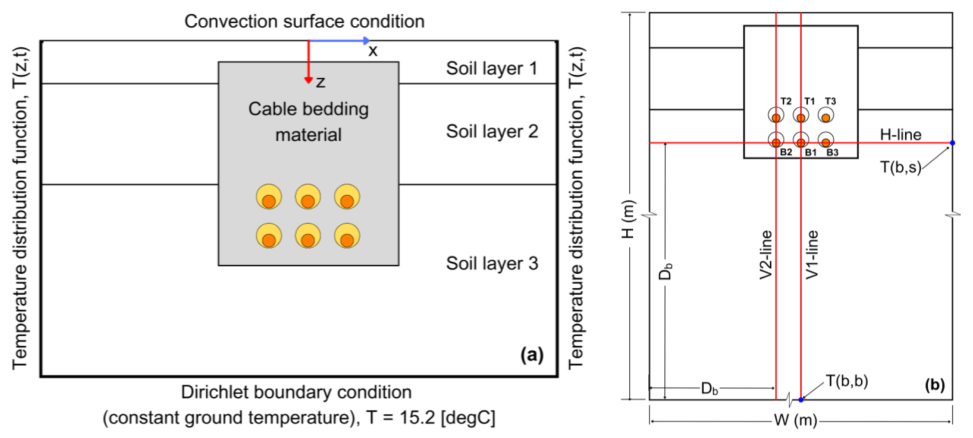
\includegraphics[width=\linewidth]{kim2025_BC}\\
\vspace{0.2em}
{\scriptsize\color{gray}
Dominio computacional: 3 capas de suelo estratificado, lecho de relleno
(bedding) y 6 cables trefoil.\\
CC superior: convección libre; CC inferior: $T=15{,}2$\,°C (Dirichlet).\\
\refcite{(Kim et al., 2025 [R5], Fig.\,7)}}

\column{0.55\textwidth}
\justifying\small
\textbf{Zonas del dominio $\Omega$}
\begin{itemize}[leftmargin=*]\scriptsize
    \item $\Omega_\text{cond}$: conductor --- fuente de calor
          $Q = I^2 R_\text{ac}$~(W/m\textsuperscript{3})
    \item $\Omega_\text{xlpe}$: aislamiento XLPE --- barrera térmica
          principal; $k\approx 0{,}286$~W/(m\,K)
    \item $\Omega_\text{bedding}$: lecho de relleno --- $k_2$
          diseñado o estimado en campo
    \item $\Omega_\text{suelo}$: suelo nativo --- $k_1(x,y)$ variable
          (principal fuente de incertidumbre)
\end{itemize}
\vspace{0.25em}
\textbf{Condiciones de contorno}
\begin{itemize}[leftmargin=*]\scriptsize
    \item $\Gamma_\text{sup}$: temperatura superficial
          $T = T_s(t)$ (Dirichlet, variación estacional)
    \item $\Gamma_\infty$: frontera lejana ---
          $T = T_\infty$ o $\partial T/\partial n = 0$
    \item Ejes de simetría:
          flujo nulo $\partial T/\partial n = 0$ (Neumann)
    \item Interfaz entre capas: continuidad de $T$ y del
          flujo térmico $k_i\nabla T\cdot\hat{n}$
\end{itemize}
\vspace{0.15em}
\textcolor{gray}{\scriptsize\refcite{(Carslaw \& Jaeger, 1959 [A13]);
(Aras et al., 2005 [R4])}}
\end{columns}
\end{frame}

% ===========================================================================
\section{Núcleo del problema}
% ===========================================================================

% ---------------------------------------------------------------------------
\begin{frame}{El problema duele: consecuencias reales de la brecha}
\begin{columns}[T]
\column{0.48\textwidth}
\begin{alertblock}{Cuando se subestima la temperatura}
\scriptsize
\begin{itemize}[leftmargin=*,itemsep=1pt]
    \item Temperatura real supera el límite del aislamiento
    \item Deterioro acelerado del XLPE (polietileno reticulado)
    \item Falla prematura, no prevista, difícil de diagnosticar
    \item Especialmente grave en cruces urbanos o zonas de alta densidad
\end{itemize}
\end{alertblock}
\column{0.48\textwidth}
\begin{exampleblock}{Cuando se sobreestima la temperatura}
\scriptsize
\begin{itemize}[leftmargin=*,itemsep=1pt]
    \item Cable opera por debajo de su capacidad real
    \item Sobredimensionamiento innecesario o subutilización del activo
    \item Pérdida de capacidad para integrar más renovables
    \item El DTR (calificación térmica dinámica) estático es conservador:
          capacidad dinámica real no aprovechada \refcite{(Fariz et al., 2026)}
\end{itemize}
\end{exampleblock}
\end{columns}

\vspace{0.2em}
\begin{columns}[T]
\column{0.48\textwidth}
\begin{block}{Diseños fuera de premisas normativas}
\scriptsize
Instalaciones con múltiples circuitos, cruces de vías o ductos en bancos se
salen de los supuestos de IEC~60287. El cálculo correcto requiere
FEM (elementos finitos) o FVM (volúmenes finitos), que no son accesibles para todos.
\refcite{(Anders, 2005, pp.~1--15); (Aras et al., 2005)}
\end{block}
\column{0.48\textwidth}
\begin{block}{Monitoreo operacional insuficiente}
\scriptsize
La mayoría de instalaciones no cuentan con sensores DTS (sensado de
temperatura distribuida por fibra óptica) ni termopares. El operador
desconoce la temperatura real y opera con incertidumbre no cuantificada.
\refcite{(Fariz et al., 2026); (Enescu et al., 2021, p.~14)}
\end{block}
\end{columns}
\end{frame}

% ---------------------------------------------------------------------------
\begin{frame}{Estado actual: métodos predominantes y sus supuestos}
\begin{columns}[T]
\column{0.48\textwidth}
\begin{alertblock}{Normas y analogía eléctrica}
\scriptsize\justifying
\textbf{IEC (Comisión Electrotécnica Internacional) 60287 / Neher-McGrath:} ampacidad en régimen
estacionario (100\% factor de carga), con $k_s$ constante, temperatura
ambiente fija y geometría estándar. Válida para el ``caso base''; menos
precisa en instalaciones complejas.
\refcite{(Neher y McGrath, 1957); (IEC 60287-1-1, 2023)}

\vspace{0.2em}
\textbf{IEC 60853 / factores de derateo:} maneja carga cíclica y
emergencias; la parte 3 considera secado parcial, pero mantiene hipótesis
fuertes de uniformidad del entorno.
\refcite{(IEC 60853-1, 1985); (IEC 60853-3, 2002)}
\end{alertblock}

\column{0.48\textwidth}
\begin{alertblock}{Modelos FEM/FDM (diferencias finitas)/FVM}
\scriptsize\justifying
Precisos y flexibles para geometrías complejas y $k(x,y)$ variable. Sin
embargo:
\begin{itemize}[leftmargin=*,itemsep=1pt]
    \item Requieren configuración experta y mallado cuidadoso
    \item Cada nueva configuración exige una nueva simulación
    \item No son prácticos para operación en tiempo real
    \item Barreras de acceso: licencias costosas, curva de aprendizaje
          lenta, tiempo de cómputo elevado
    \item No diseñados para el \textit{problema inverso} (estimar
          $k$ desde mediciones)
\end{itemize}
\refcite{(Aras et al., 2005); (CIGRÉ WG B1.56, 2022)}
\end{alertblock}
\end{columns}

\vspace{0.2em}
\refcite{(Anders, 2005); (Al-Dulaimi et al., 2024, p.~2)}
\end{frame}

% ---------------------------------------------------------------------------
\begin{frame}{Estado actual: casos donde los métodos vigentes fallan}

\begin{columns}[T]
\column{0.48\textwidth}

\begin{block}{Cruces y entornos de alta densidad}
\small Múltiples circuitos, cables en bancos o ductos, cruces de vías.
La interacción térmica entre cables y la variabilidad del relleno superan
las premisas de las normas. FEM es el camino pero no suele implementarse.
\refcite{(Anders, 2005, pp.~50--80); (Atoccsa et al., 2024)}
\end{block}
\vspace{0.3em}
\begin{block}{Variación estacional y climática}
\small La temperatura del suelo varía entre verano e invierno; la humedad
cambia con las lluvias. La ampacidad real no es fija sino variable durante
el año. Los ratings estáticos no capturan esto.
\refcite{(Möbius et al., 2025); (Kim et al., 2025)}
\end{block}

\column{0.48\textwidth}

\begin{block}{Secado térmico local}
\small Bajo carga sostenida, el suelo cerca del cable se seca, su
resistividad sube de 1.0 a más de 2.5 K·m/W, y la temperatura del
conductor aumenta de forma no lineal y no capturada por los modelos
estáticos. \refcite{(Khumalo et al., 2025, pp.~6--10)}
\end{block}
\vspace{0.3em}
\begin{block}{DTR en cargas fluctuantes}
\small Para energía renovable la carga varía continuamente. Los modelos de
red térmica equivalente pierden precisión bajo variaciones rápidas. Se
necesita un modelo dinámico robusto.
\refcite{(Enescu et al., 2021, pp.~8--12); (Fariz et al., 2026)}
\end{block}
\end{columns}
\end{frame}

% ---------------------------------------------------------------------------
\begin{frame}{Estado deseable}
\begin{exampleblock}{¿Cómo debería ser?}
\justifying\small
Contar con un modelo computacional de la transferencia de calor en cables
subterráneos que sea capaz de:
\begin{itemize}[leftmargin=*]
    \item representar geometrías e instalaciones complejas con conductividad
          térmica variable por zonas $k(x,y)$, sin supuestos de uniformidad;
    \item resolver el \textbf{problema directo} (temperatura dada la carga y
          el entorno) y el \textbf{problema inverso} (estimar $k$ del suelo o
          backfill desde mediciones de temperatura operativa);
    \item ser \textbf{adaptable} para distintas configuraciones de diseño sin
          reconfiguración experta compleja;
    \item ser \textbf{eficiente} para escenarios de diseño, optimización,
          DTR y mantenimiento predictivo (no solo para simulación estática);
    \item ser \textbf{validable} con casos de referencia publicados
          (CIGRÉ [Consejo Internacional de Grandes Redes Eléctricas] WG~B1.56, literatura) y con código abierto y reproducible;
    \item poder \textbf{integrarse con señales operacionales} (sensores,
          SCADA [control supervisorio y adquisición de datos]) para actualización de parámetros y estimación de temperatura
          en tiempo real o cuasi-real.
\end{itemize}
\end{exampleblock}
\vspace{0.2em}
\refcite{(Fariz et al., 2026); (CIGRÉ WG B1.56, 2022); (Al-Dulaimi et al., 2024);
(Billah et al., 2023)}
\end{frame}

% ---------------------------------------------------------------------------
\begin{frame}{La brecha: de dónde venimos y a dónde queremos llegar}

\begin{center}
\resizebox{\textwidth}{!}{%
\begin{tikzpicture}[>=Stealth,
  estado/.style={draw, rounded corners=4pt, text width=3.6cm,
                 align=center, minimum height=2.8cm, font=\small,
                 inner sep=6pt},
  lbl/.style={font=\tiny\bfseries, text width=3.4cm, align=center}]

  \node[estado, fill=red!12, draw=red!60!black] (actual) at (0,0) {
    \textbf{Estado actual}\\[4pt]
    \footnotesize
    Normas IEC/Neher-McGrath\\
    con supuestos uniformes\\[2pt]
    FEM complejo, no accesible\\[2pt]
    Sin inversión de parámetros\\[2pt]
    Sin real-time\\[2pt]
    Incertidumbre en $T_\text{cond}$
  };

  \node[estado, fill=orange!18, draw=orange!70!black] (brecha) at (5.2,0) {
    \textbf{Brecha}\\[4pt]
    \footnotesize
    Heterogeneidad térmica\\
    $k(x,y)$ ignorada o\\
    asumida constante\\[2pt]
    Casos complejos fuera\\
    de premisas normativas\\[2pt]
    Sin herramienta abierta\\
    y adaptable\\[2pt]
    Incapacidad predictiva
  };

  \node[estado, fill=green!10, draw=green!50!black] (deseable) at (10.4,0) {
    \textbf{Estado deseable}\\[4pt]
    \footnotesize
    Modelo 2D con $k(x,y)$\\
    variable por zonas\\[2pt]
    Problema directo\\
    e inverso resueltos\\[2pt]
    Adaptable, open-source\\[2pt]
    Eficiente para DTR\\
    y mantenimiento\\[2pt]
    Validado con literatura
  };

  \draw[->, very thick, red!70!black] (actual.east) -- (brecha.west);
  \draw[->, very thick, dashed, green!60!black]
        (brecha.east) -- node[above, font=\tiny, color=green!40!black]
        {cerrar} (deseable.west);

  \node[lbl, below=0.25cm of actual, text=red!70!black]
        {Métodos insuficientes\\para condiciones reales};
  \node[lbl, below=0.25cm of brecha, text=orange!80!black]
        {Problema a resolver\\(esta investigación)};
  \node[lbl, below=0.25cm of deseable, text=green!50!black]
        {Meta: mayor precisión,\\seguridad y eficiencia};
\end{tikzpicture}%
}
\end{center}
\end{frame}

% ---------------------------------------------------------------------------
\begin{frame}{Formulación del problema}
\begin{exampleblock}{Síntesis}
\justifying\small
Los métodos predominantes de evaluación térmica de cables eléctricos
subterráneos ---basados en normas estacionarias (IEC~60287, IEC~60853,
Neher-McGrath) o en modelos FEM de uso restringido--- asumen condiciones
térmicas homogéneas y no están diseñados para representar la heterogeneidad
real del suelo, los casos de instalación complejos ni la estimación inversa
de propiedades térmicas desde mediciones operativas. Esta limitación genera
una \textbf{brecha} entre la temperatura estimada del conductor y la
temperatura real bajo condiciones de suelo variable, secado térmico, cargas
dinámicas o arreglos de múltiples circuitos. La brecha se expresa como
incertidumbre sobre la ampacidad disponible, riesgo de sobrecalentamiento
no detectado, y falta de herramientas accesibles para el diseño y la
operación de instalaciones fuera del caso base normativo. Cerrar esta brecha
permitiría diseñar instalaciones más seguras, operar sistemas con mayor
aprovechamiento de la capacidad térmica real, y habilitar el mantenimiento
predictivo de activos críticos sin redundancia.
\end{exampleblock}

\vspace{0.3em}
\refcite{(Neher y McGrath, 1957); (IEC 60287-1-1, 2023); (Aras et al., 2005);
(Khumalo et al., 2025); (Enescu et al., 2021); (Fariz et al., 2026);
(Anders, 2005)}
\end{frame}

% ===========================================================================
\section{Preguntas y objetivos}
% ===========================================================================

\begin{frame}{Pregunta de investigación}

\begin{block}{Pregunta central}
\justifying
¿En qué medida los métodos simplificados de evaluación térmica de cables
eléctricos subterráneos representan adecuadamente la distribución de
temperatura real cuando el suelo presenta conductividad térmica
espacialmente variable $k(x,y)$, y cuál es el efecto cuantificable
de dicha variabilidad sobre la temperatura máxima del conductor y la
ampacidad estimada?
\end{block}

\vspace{0.7em}
\textbf{Preguntas subordinadas:}
\begin{itemize}[leftmargin=*]\small
    \item ¿Cuáles son los supuestos de IEC~60287 y del método
          Neher-McGrath que limitan su validez bajo condiciones reales
          de suelo y de instalación?
    \item ¿Cuánto varía la temperatura del conductor al cambiar la
          distribución espacial de $k(x,y)$ del suelo y del material
          de relleno?
    \item ¿Qué configuraciones de instalación se alejan más de las
          premisas normativas y generan mayor incertidumbre?
    \item ¿Qué información operativa y qué tipo de modelo serían
          necesarios para estimar la ampacidad dinámica real con mayor
          precisión?
\end{itemize}
\end{frame}

% ---------------------------------------------------------------------------
\begin{frame}{Objetivos}

\begin{block}{Objetivo general}
\justifying\small
Caracterizar y cuantificar la brecha entre los métodos normativos
simplificados y el comportamiento térmico real de cables eléctricos
subterráneos, identificando las condiciones de suelo, geometría de
instalación y perfil de carga que determinan la magnitud de dicha
brecha y los requisitos para cerrarla.
\end{block}

\vspace{0.5em}
\textbf{Objetivos específicos:}
\begin{enumerate}[leftmargin=*]\small
    \item Describir y sistematizar los supuestos y limitaciones de los
          métodos normativos vigentes (IEC 60287, IEC 60853, Neher-McGrath)
          para el cálculo de ampacidad en condiciones no ideales.
    \item Identificar los casos de instalación o condición de entorno donde
          los métodos simplificados presentan mayor desviación respecto a
          modelos numéricos más detallados.
    \item Analizar cuantitativamente el efecto de la variabilidad de
          propiedades térmicas del suelo/backfill $[k(x,y),\;\rho c(x,y)]$
          sobre $T_{\max}$ del conductor y la ampacidad estimada.
    \item Delimitar los requisitos funcionales de un modelo computacional
          abierto para representar adecuadamente la transferencia de calor
          bidimensional con $k(x,y)$ variable y condiciones de instalación
          complejas.
\end{enumerate}
\end{frame}

% ---------------------------------------------------------------------------
\begin{frame}{Esbozo de posibles enfoques de solución (preliminar)}
\justifying\scriptsize
El problema identificado orienta hacia las siguientes posibilidades
\textbf{(no es metodología aún; se define en etapas posteriores):}

\vspace{0.15em}
\begin{columns}[T]
\column{0.48\textwidth}
\begin{block}{Modelado numérico directo}
\scriptsize FEM o FVM en Python (FEniCSx, FreeFEM) para resolver
$\nabla\cdot(k\nabla T) + Q = 0$ con $k(x,y)$ variable.
Permite validar contra IEC~60287 y cuantificar la brecha en distintos
escenarios. \refcite{(Aras et al., 2005); (CIGRÉ WG B1.56, 2022)}
\end{block}
\vspace{0.15em}
\begin{block}{PINNs (redes neuronales informadas por física) --- directo e inverso}
\scriptsize Incorporan la PDE (ecuación diferencial parcial) en la función de pérdida. Pueden estimar $k(x,y)$
del suelo desde mediciones de temperatura (problema inverso), sin necesidad
de re-mallado.
\refcite{(Raissi et al., 2019); (Billah et al., 2023)}
\end{block}
\column{0.48\textwidth}
\begin{block}{Surrogate o metamodelo paramétrico}
\scriptsize Modelo entrenado para evaluar rápidamente $T_{\max}$ ante cambios
de geometría, material y condiciones, sin correr FEM desde cero.
Útil para diseño de bedding/backfill y optimización de ampacidad.
\refcite{(Ocłoń et al., 2015); (Atoccsa et al., 2024)}
\end{block}
\vspace{0.15em}
\begin{block}{Gemelo térmico operacional}
\scriptsize Modelo que se actualiza con datos de sensores (DTS, SCADA) para
estimar temperatura del conductor en cuasi-tiempo real y soportar
mantenimiento predictivo y DTR.
\refcite{(Fariz et al., 2026); (Al-Dulaimi et al., 2024)}
\end{block}
\end{columns}
\end{frame}

% ---------------------------------------------------------------------------
\begin{frame}{Alta fidelidad del modelo PINN vs.\ FEM de referencia}
\centering
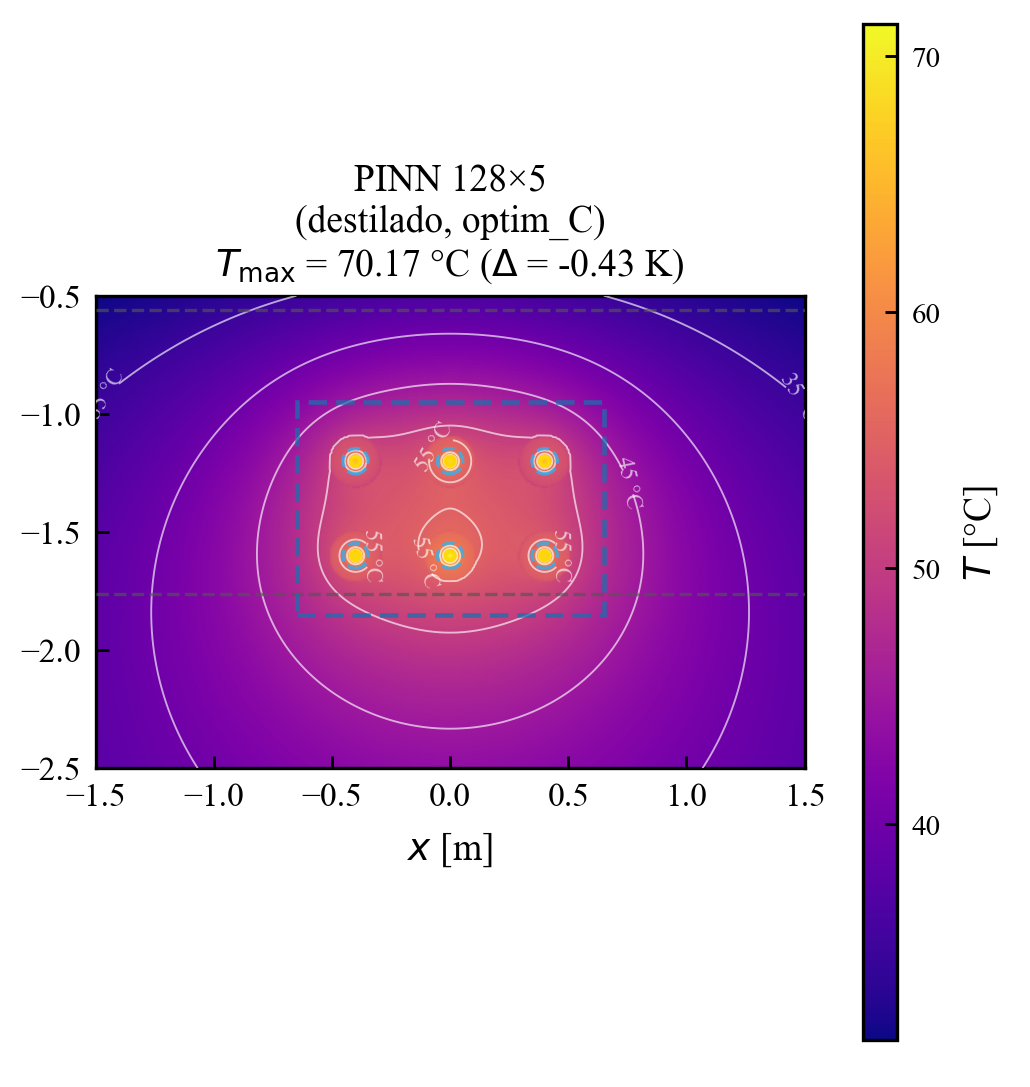
\includegraphics[width=0.88\linewidth]{own_kim_fem_zoom}\\
\vspace{0.3em}
\small 4 paneles: campo $T$ del FEM de referencia y tres variantes PINN
(Kim et al.\ 2025, Caso B).
$|\Delta T|_{\max} < 0{,}5$~K entre FEM y la mejor variante PINN.\\
\vspace{0.2em}
\refcite{Kim et al.\ (2025) [R5]; resultados propios.}
\end{frame}

% ===========================================================================
\section{Referencias}
% ===========================================================================

% ---- Refs R1-R3 -----------------------------------------------------------
\begin{frame}{Referencias principales (1/7)}
\small\justifying

\textbf{[R1]} Neher, J. H., \& McGrath, M. H. (1957). The calculation of the
temperature rise and load capability of cable systems. \textit{AIEE Trans.
III: Power Apparatus and Systems, 76}(3), 752--772.\\
\textcolor{blue!60!black}{\footnotesize\textit{Tipo: Aporte fundamental}} \quad
\textcolor{gray}{\footnotesize Base matemática del cálculo de ampacidad; define
los supuestos del estado actual que esta investigación busca superar.}

\medskip
\textbf{[R2]} International Electrotechnical Commission. (2023). \textit{IEC
60287-1-1:2023 -- Electric cables -- Calculation of the current rating.} IEC.\\
\textcolor{blue!60!black}{\footnotesize\textit{Tipo: Norma vigente}} \quad
\textcolor{gray}{\footnotesize Estándar internacional para ampacidad estacionaria;
sus supuestos de uniformidad térmica son la principal limitación que se
caracteriza en esta investigación.}

\medskip
\textbf{[R3]} Anders, G. J. (2005). \textit{Rating of electric power cables in
unfavorable thermal environment.} IEEE Press / Wiley.\\
\textcolor{blue!60!black}{\footnotesize\textit{Tipo: Libro de referencia (estado del arte)}} \quad
\textcolor{gray}{\footnotesize Extiende IEC~60287 a entornos con resistividad
elevada, secado térmico y configuraciones complejas; referencia estándar de la
industria para los límites del enfoque normativo.}
\end{frame}

% ---- Refs R4-R6 -----------------------------------------------------------
\begin{frame}{Referencias principales (2/7)}
\small\justifying

\textbf{[R4]} Aras, F., Oysu, C., \& Yilmaz, G. (2005). An assessment of the
methods for calculating ampacity of underground power cables. \textit{Electric
Power Components and Systems, 33}(12), 1385--1402.\\
\textcolor{blue!60!black}{\footnotesize\textit{Tipo: Estado del arte / comparación de métodos}} \quad
\textcolor{gray}{\footnotesize Compara sistemáticamente métodos normativos y FEM;
base empírica para justificar la brecha entre modelos simplificados y
condiciones reales de instalación.}

\medskip
\textbf{[R5]} Kim, Y.-S. et al. (2025). Effect of ambient air and ground
temperatures on heat transfer in underground power cable system buried in newly
developed cable bedding material. \textit{Geothermics, 125}, 103151.\\
\textcolor{blue!60!black}{\footnotesize\textit{Tipo: Aplicación / estudio experimental-numérico}} \quad
\textcolor{gray}{\footnotesize Cuantifica el efecto del material de bedding y la
temperatura del suelo sobre $T_{\text{cond}}$; evidencia directa de la
influencia de $k(x,y)$ (\textbf{X}) sobre la temperatura (\textbf{Y}).}

\medskip
\textbf{[R6]} Khumalo, N. Q. et al. (2025). A critical assessment of cable
rating methods under soil drying out conditions. \textit{Int. Trans. Electrical
Energy Systems.}\\
\textcolor{blue!60!black}{\footnotesize\textit{Tipo: Análisis crítico / estado del arte}} \quad
\textcolor{gray}{\footnotesize Demuestra que el secado del suelo eleva la
resistividad térmica y degrada la ampacidad; señala los límites de IEC~60853-3.}
\end{frame}

% ---- Refs R7-R9 -----------------------------------------------------------
\begin{frame}{Referencias principales (3/7)}
\small\justifying

\textbf{[R7]} Enescu, D. et al. (2021). Concepts and methods to assess the
dynamic thermal rating of underground power cables. \textit{Energies,
14}(9), 2591.\\
\textcolor{blue!60!black}{\footnotesize\textit{Tipo: Revisión sistemática (DTR)}} \quad
\textcolor{gray}{\footnotesize Revisa exhaustivamente los métodos DTR; subraya
que la resistividad del suelo y los modelos estáticos son las principales
fuentes de incertidumbre en la temperatura del conductor.}

\medskip
\textbf{[R8]} Fariz, K. et al. (2026). A systematic mapping of dynamic thermal
rating for underground cables. \textit{IEEE Access.}\\
\textcolor{blue!60!black}{\footnotesize\textit{Tipo: Revisión sistemática / mapeo 2020--2026}} \quad
\textcolor{gray}{\footnotesize Identifica brechas metodológicas abiertas en DTR
de cables subterráneos; referencia más reciente del estado del arte e hilo
conductor para justificar la relevancia del problema.}

\medskip
\textbf{[R9]} Raissi, M., Perdikaris, P., \& Karniadakis, G. E. (2019).
Physics-informed neural networks: A deep learning framework for solving forward
and inverse problems involving nonlinear PDEs. \textit{J. Computational
Physics, 378}, 686--707.\\
\textcolor{blue!60!black}{\footnotesize\textit{Tipo: Aporte fundamental (PINNs)}} \quad
\textcolor{gray}{\footnotesize Introduce el marco PINN: integra la PDE (ecuación
de calor) en la función de pérdida; base metodológica para el enfoque directo
e inverso propuesto en esta investigación.}
\end{frame}

% ---- Refs R10, A1, A2 -----------------------------------------------------
\begin{frame}{Referencias adicionales (4/7)}
\small\justifying

\textbf{[R10]} Lawal, Z. K. et al. (2022). Physics-informed neural network
(PINN) evolution and beyond: a systematic literature review and bibliometric
analysis. \textit{Big Data and Cognitive Computing, 6}(4), 140.\\
\textcolor{blue!60!black}{\footnotesize\textit{Tipo: Revisión sistemática (PINNs)}} \quad
\textcolor{gray}{\footnotesize Revisa la evolución y variantes de PINNs
(XPINNs, cPINNs); sustenta la madurez tecnológica del enfoque como solución
viable para el problema de la investigación.}

\medskip
\textbf{[A1]} Incropera, F. P., \& DeWitt, D. P. (2011). \textit{Fundamentals
of Heat and Mass Transfer} (7th ed.). Wiley.\\
\textcolor{purple!70!black}{\footnotesize\textit{Tipo: Libro de referencia fundamental (transferencia de calor)}} \quad
\textcolor{gray}{\footnotesize Presenta la ecuación de calor estacionaria
$\nabla\cdot(k\nabla T)+Q=0$ y transitoria $\rho c_p \partial T/\partial t =
\nabla\cdot(k\nabla T)+Q$; marco físico central del problema de investigación.}

\medskip
\textbf{[A2]} Ocłoń, P. et al. (2015). Optimizing of the underground power
cable bedding using momentum-type particle swarm optimization. \textit{Energy,
92}(P2), 230--239.\\
\textcolor{purple!70!black}{\footnotesize\textit{Tipo: Aplicación / optimización}} \quad
\textcolor{gray}{\footnotesize Optimiza el material de bedding para minimizar
$T_{\text{cond}}$; evidencia que variar $k$ del relleno tiene impacto
cuantificable sobre la temperatura del conductor.}
\end{frame}

% ---- Refs A3-A5 -----------------------------------------------------------
\begin{frame}{Referencias adicionales (5/7)}
\small\justifying

\textbf{[A3]} Al-Dulaimi, A. et al. (2024). Adaptive FEM-BPNN model for
predicting underground cable temperature considering varied soil composition.
\textit{Engineering Science and Technology.}\\
\textcolor{purple!70!black}{\footnotesize\textit{Tipo: Aplicación (FEM + IA)}} \quad
\textcolor{gray}{\footnotesize Combina FEM y redes neuronales para predecir
$T_{\text{cond}}$ según la composición del suelo; referente directo de la
línea solución numérico-inteligente propuesta.}

\medskip
\textbf{[A4]} Atoccsa, B. et al. (2024). Optimization of ampacity in HV
underground cables with thermal backfill using dynamic PSO and adaptive
strategies. \textit{Energies, 17}(5), 1023.\\
\textcolor{purple!70!black}{\footnotesize\textit{Tipo: Aplicación / optimización de diseño}} \quad
\textcolor{gray}{\footnotesize Demuestra que ajustar el backfill mejora la
ampacidad; relaciona directamente $k(x,y)$ (\textbf{X}) con la temperatura
del conductor (\textbf{Y}) bajo carga.}

\medskip
\textbf{[A5]} Möbius, P. et al. (2025). Energy cable ampacity: impact of
seasonal and climate-related changes. \textit{Renewable and Sustainable Energy
Reviews.}\\
\textcolor{purple!70!black}{\footnotesize\textit{Tipo: Estado del arte / impacto climático}} \quad
\textcolor{gray}{\footnotesize Cuantifica cómo la variación estacional de la
temperatura del suelo y la humedad afectan la ampacidad real; justifica la
necesidad de modelos dinámicos que superen las normas estáticas.}
\end{frame}

% ---- Refs A6-A8 -----------------------------------------------------------
\begin{frame}{Referencias adicionales (6/7)}
\small\justifying

\textbf{[A6]} Billah, M. M. et al. (2023). Physics-informed deep neural
network for inverse heat transfer problems in materials. \textit{Materials
Today Communications, 35}, 106336.\\
\textcolor{purple!70!black}{\footnotesize\textit{Tipo: Aplicación (PINN inverso)}} \quad
\textcolor{gray}{\footnotesize Resuelve el problema inverso de transferencia de
calor con PINNs; referente metodológico directo para estimar $k(x,y)$ del
suelo desde mediciones de temperatura del cable.}

\medskip
\textbf{[A7]} CIGRÉ Working Group B1.56. (2022). \textit{Power cable rating
examples for calculation tool verification.} CIGRÉ.\\
\textcolor{purple!70!black}{\footnotesize\textit{Tipo: Documento técnico / benchmark}} \quad
\textcolor{gray}{\footnotesize Proporciona casos de validación para herramientas
de cálculo de ampacidad; referencia clave para verificar los modelos
numéricos desarrollados en la investigación.}

\medskip
\textbf{[A8]} IEC 60853-3:2002. \textit{Calculation of the cyclic and
emergency current rating of cables -- Part 3: Cyclic rating factor with
partial drying of the soil.} IEC.\\
\textcolor{purple!70!black}{\footnotesize\textit{Tipo: Norma técnica}} \quad
\textcolor{gray}{\footnotesize Extiende el cálculo de derateo cíclico al caso
de secado parcial del suelo; delimita el alcance normativo actual y la
brecha que se busca cerrar.}
\end{frame}

% ---- Refs A9-A11 ----------------------------------------------------------
\begin{frame}{Referencias adicionales (7/7)}
\small\justifying

\textbf{[A9]} Kolawole, O. et al. (2024). Evaluating soil thermal
conductivity for buried infrastructure. \textit{Progress in Engineering
Science.}\\
\textcolor{purple!70!black}{\footnotesize\textit{Tipo: Estudio experimental}} \quad
\textcolor{gray}{\footnotesize Mide $k$ del suelo bajo distintas condiciones de
salinidad, humedad y composición mineral; aporta datos empíricos para la
variable $X$ del problema.}

\medskip
\textbf{[A10]} CIGRÉ Working Group B1.87. (2025). \textit{Finite element
analysis for cable rating calculations.} CIGRÉ.\\
\textcolor{purple!70!black}{\footnotesize\textit{Tipo: Documento técnico (FEM aplicado)}} \quad
\textcolor{gray}{\footnotesize Guía oficial de CIGRÉ para aplicar FEM al cálculo
de ampacidad; referente para validar y contextualizar el modelado numérico
propuesto.}

\medskip
\textbf{[A11]} Pan, Y. et al. (2025). Reconstruction of the temperature field
in 2D steady-state thermal conductivity based on PINNs. \textit{Eng,
6}(5), 99.\\
\textcolor{purple!70!black}{\footnotesize\textit{Tipo: Aplicación (PINN 2D)}} \quad
\textcolor{gray}{\footnotesize Reconstruye el campo de temperatura 2D en un
dominio con $k$ variable usando PINNs; caso directamente análogo al problema
de esta investigación, con geometría y ecuación gobernante equivalentes.}

\medskip
\textbf{[A12]} Thue, W. A. (2012). \textit{Electrical Power Cable Engineering}
(3rd ed.). CRC Press / Taylor \& Francis.\\
\textcolor{purple!70!black}{\footnotesize\textit{Tipo: Libro de referencia (ingeniería de cables)}} \quad
\textcolor{gray}{\footnotesize Describe la estructura, propiedades térmicas y
eléctricas de cables de potencia; base para caracterizar capas, fuentes de calor
($I^2 R$, pérdidas dieléctricas, corrientes de pantalla) y límites operativos
del aislamiento XLPE.}

\medskip
\textbf{[A13]} Carslaw, H. S., \& Jaeger, J. C. (1959). \textit{Conduction of
Heat in Solids} (2nd ed.). Oxford University Press.\\
\textcolor{purple!70!black}{\footnotesize\textit{Tipo: Libro de referencia fundamental (transferencia de calor)}} \quad
\textcolor{gray}{\footnotesize Formulación matemática clásica de la conducción
de calor estacionaria y transitoria; fundamento teórico de la ecuación que
gobierna el campo térmico en cables y suelo.}
\end{frame}



% ---------------------------------------------------------------------------
\begin{frame}
\centering
{\Large \textbf{Gracias}}

\vspace{1.0em}
\large Luis Koc \quad $|$ \quad Herbert Meléndez

\vspace{0.5em}
\normalsize Trabajo de Investigación I $\cdot$ MIA 3er Ciclo A 2026-1

\vspace{0.8em}
\begin{block}{\centering Síntesis del problema}
\centering\small
Existe una brecha entre los métodos simplificados de evaluación térmica de
cables subterráneos y la realidad del sistema bajo condiciones heterogéneas,
dinámicas y complejas. Cerrar esa brecha requiere modelos más representativos,
adaptables y accesibles que permitan mejor diseño, operación segura y
mantenimiento predictivo de infraestructura crítica.
\end{block}
\end{frame}

\end{document}
